% Created 2022-12-18 Sun 20:51
% Intended LaTeX compiler: pdflatex
\documentclass[11pt]{article}
\usepackage[utf8]{inputenc}
\usepackage[T1]{fontenc}
\usepackage{graphicx}
\usepackage{longtable}
\usepackage{wrapfig}
\usepackage{rotating}
\usepackage[normalem]{ulem}
\usepackage{amsmath}
\usepackage{amssymb}
\usepackage{capt-of}
\usepackage{hyperref}
\usepackage{todonotes}
\usepackage[portuges]{babel}
\usepackage{amsthm}
\usepackage[a4paper, total={6in, 8in}]{geometry}
\author{Ieremies V. F. Romero}
\date{\today}
\title{Projeto 2 - MO420}
\hypersetup{
 pdfauthor={Ieremies V. F. Romero},
 pdftitle={Projeto 2 - MO420},
 pdfkeywords={},
 pdfsubject={},
 pdfcreator={Emacs 28.2 (Org mode 9.6)}, 
 pdflang={Portuges}}
\usepackage{biblatex}
\addbibresource{~/arq/bib.bib}
\begin{document}

\maketitle

\section{Problema}
\label{sec:orgfc61a70}
Neste projeto, estudaremos o problema conhecido como \emph{Travelling Sales Man with Drone} (TSP-D). Assim como no TSP clássico, temos um digrafo \(G = (V,A)\) e queremos visitar todos os nós. Porém, neste caso, dispomos de um caminhão e um drone que pode auxiliar nas visitas. O drone deve partir e voltar para o caminhão após cada visita e esta deve respeitar o limite de distância \(D\) do drone. O caminhão parte do nó \(s\) e deve terminar, com o drone, no nó \(t\). Nosso objetivo é minimizar a soma dos custos do caminhão (\(c_{ij}\)) e do drone (\(d_{ij}\)).

Assim, uma solução para o problema é composta de um caminho de \(s\) a \(t\) descrito por \(P = (V_P, A_P)\) e de um conjunto de arcos \(B\). \(V_P \subseteq V\) é o conjunto de nós do caminho \(P\) e \(A_P \subseteq A\) o conjunto de arcos que o compõe. Já o conjunto \(B \subseteq V \setminus V_p \times V_P\) é um conjunto que se \((i,j) \in B\), então \((i,j) \notin A_P\) (e \((j,i) \notin A\)) e \(d_{ij} + d_{ji} \leq D\). Além disso, para cada nó \(i \in V \setminus V_P\) há exatamente um par \((i,j) \in B\), para algum \(j \in V_P\).

\section{Formulação Inteira}
\label{sec:org3c974d7}
Seja \(V' = V \setminus \{s,t\}\). Usaremos \(2\) variáveis binárias:
\begin{itemize}
\item \(x_{ij}\) é igual a \(1\) se, e somente se, o caminhão percorre a aresta \((i,j) \in A\).
\item \(y_{ij}\) é igual a \(1\) se, e somente se, o drone percorre a aresta \((i,j) \in A\).
\end{itemize}

Além disso, usaremos as variáveis \(u_i\) para atribuir um peso ao nó \(i\) para evitar ciclos do caminhão.

\begin{alignat}{4}
& \omit\rlap{minimize  $\displaystyle \sum_{i \in V} \sum_{j \in V ,j \neq i} x_{ij} c_{ij} + y_{ij} d_{ij} $} \\
& \mbox{sujeito a}&& \quad & \sum_{i \in V'} x_{si} &= \sum_{i \in V'} x_{it} = 1                 & \quad &  \\
&                 &&       &  \sum_{i \in V'} x_{is} &= \sum_{i \in V'} x_{ti} = 0                 & \quad &  \\
&                 &&       & \sum_{j \in V', j \neq i} x_{ji} &= \sum_{j \in V', j \neq i} x_{ij}     &       & \forall i \in V'   \\
&                 &&       & a_i + c_{ij} &\leq a_j + M(1 - x_{ij})                             &       & \forall i,j \in V \\
&                 &&       & y_{ij} &= y_{ji}                                                   &       & \forall i,j \in V   \\
&                 &&       & \sum_{k \in V', k \neq i} x_{ki} &\geq y_{ij}                                &       & \forall i,j \in V' \\
&                 &&       & \sum_{j \in V, j \neq i} x_{ij} + y_{ij} &\geq 1                        &       & \forall i \in V   \\
&                 &&       & y_{ij} c_{ij} + y_{ji} c_{ji} &\leq D                               &       & \forall i,j \in V  \\
&                 &&       & x_{ij} y_{ij} &\in \{0,1\}                                         &       & \forall i,j \in V \\
&                 &&       & a_i &\in \mathbb{R}_+                                             &         & \forall i \in V
\end{alignat}

Nossa função objetivo é bem direta: soma dos custos do caminhão e do drone. Restrição \(2\) e \(3\) garantem que o caminhão irá partir de \(s\) e chegar em \(t\). Restrição \(4\) garante a manutenção de fluxo enquanto restrição \(5\) evita ciclos. Restrição \(6\) garante que toda viagem do drone irá voltar para o nó que partiu e restrição \(7\) garante que ele só partirá de um nó visitado pelo caminhão. Restrição \(8\) garante que todos os nós serão visitados, ou pelo caminhão, ou pelo drone. Restrição \(9\) força que as viagens do drone respeitem seu limite de distância. Por fim, restrições \(10\) e \(11\) definem o domínio das variáveis.

\section{\emph{Branch-and-cut}}
\label{sec:orgd00a974}
Apesar da formulação acima funcionar, se observarmos a literatura para o \textbf{Problema do Caxeiro Viajante} (TSP), formulações que usam elminação de subciclo tendem a ter performance melhores na prática.
\begin{alignat}{4}
& \omit\rlap{minimize  $\displaystyle \sum_{i \in V} \sum_{j \in V ,j \neq i} x_{ij} c_{ij} + y_{ij} d_{ij} $} \\
& \mbox{sujeito a}&& \quad & \sum_{i \in V'} x_{si} &= \sum_{i \in V'} x_{it} = 1                 & \quad &  \\
&                 &&       &  \sum_{i \in V'} x_{is} &= \sum_{i \in V'} x_{ti} = 0                 & \quad &  \\
&                 &&       & \sum_{j \in V', j \neq i} x_{ji} &= \sum_{j \in V', j \neq i} x_{ij}     &       & \forall i \in V'   \\
&                 &&       & \sum_{i \in M} \sum_{j \in M} x_{ij} &\leq |M| -1                                        &       & \forall M \subseteq V /\{s\} \\
&                 &&       & y_{ij} &= y_{ji}                                                   &       & \forall i,j \in V   \\
&                 &&       & \sum_{k \in V', k \neq i} x_{ki} &\geq y_{ij}                                &       & \forall i,j \in V' \\
&                 &&       & \sum_{j \in V, j \neq i} x_{ij} + y_{ij} &\geq 1                        &       & \forall i \in V   \\
&                 &&       & y_{ij} c_{ij} + y_{ji} c_{ji} &\leq D                               &       & \forall i,j \in V  \\
&                 &&       & x_{ij} y_{ij} &\in \{0,1\}                                         &       & \forall i,j \in V \\
&                 &&       & a_i &\in \mathbb{R}_+                                             &         & \forall i \in V
\end{alignat}

Nessa formulação, restringimos que para todos os subconjuntos de vértices, a quantidade de arestas utilizadas seja menor que o tamanho do subconjunto, chamadas des restrições de subciclos.
O problema agora é que possuímos uma quantidade exponencial de restrições.
Para tal, utilizaremos a estratégia de \emph{branch-and-cut} onde resolvemos a formulação sem as restrições de subciclos.
Possívelmente, a solução obtida violará alguma destas restrições e nosso trabalho reside em determinar qual é e adiciona-la, resolvendo novamente.
Realizamos esse processo até que nenhuma seja violada.

Nesse trabalho, testamos duas ``estratégias'' de corte. A primeira estratégia concistia em ``cortar'' apenas o ciclo em específico que aparece na solução. Já a segunda estratégia, adicionamos a restrição exatamente como descrito na formulação acima.

O algortimo para achar um subciclo é apresentado abaixo.

\begin{verbatim}
bool found = false;   // se um subciclo foi achado
vector<Arc> subcycle; // o caminho atual

for (DNodeIt o(drone.dg); o != INVALID and !found; ++o) {
    // Inicializa as estruturas necessárias
    DNodeBoolMap visited(drone.dg, false);
    subcycle.clear();

    // Nó inicial
    DNode n = o;
    visited[n] = true;

    // Caminha pelo grafo
    for (Arc a = next(n); a != INVALID and !found; a = next(n)) {
    subcycle.push_back(a);
    n = drone.dg.target(a);

    // Se voltarmos para alguém já visitado, achamos um subciclo
    if (visited[n])
        found = true;
    visited[n] = true;
    }
}
\end{verbatim}

\section{Resultados}
\label{sec:org56453a8}
Para esse projeto, foram utilizadas as novas instâncias disponibilizadas pelo professor. Os experimentos foram realizados num LG Gram equipado com um Intel Core i5 de 8ª geração, quad-core, 1.6GHz, 8GB de memória ram. A máquina estava equipada com Linux Manjaro e sendo utilizado o solver Gurobi versão 9.5.2.

Na tabela do Apendíce encontram-se os resultados do experimento. A coluna número de nós (\texttt{nnodoes}) se refere a quantidade de nós visitados na árvore de branch-and-bound. Utilizamos como tempo limite \(300\) segundos.

Para melhor visualizar o impacto das estratégias de \emph{branch-and-cut}, fica melhor visualizarmos a partir de um \emph{Performance Profile}, como proposto por \textcite{Dolan2002Benchmarkingoptimizationsoftware}, na Figura \ref{fig:perf_profile}.

\begin{figure}[htbp]
\centering
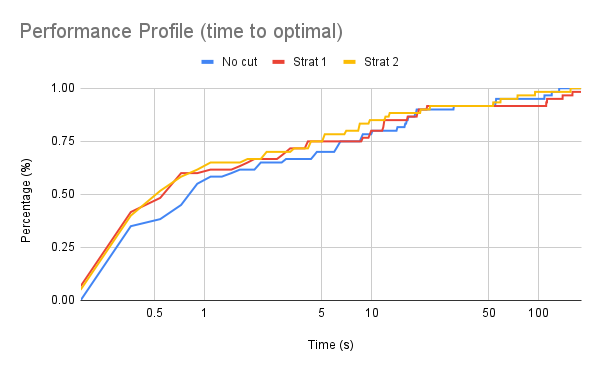
\includegraphics[width=.9\linewidth]{./pp.png}
\caption{\label{fig:perf_profile}Performance profile do tempo para atingir o ótimo da instância. ``No cut'' é a curva correspondente à formulação simples, ``strat 1'' com a primeira estratégia e ``strat 2'' a segunda.}
\end{figure}

A partir da Figura \ref{fig:perf_profile} podemos observar que a primeira estratégia de corte não foi suficiente para melhorar, claramente ficando atrás da opção sem \emph{branch-and-cut}. Por sua vez, a segunda estratégia já se mostrou concistentemente melhor ou tão bom quanto, sendo assim uma opção mais sólida. Além disso, observando as tabelas, vemos que a quantidade de nós na árvore de \emph{branch-and-bound} é consideravelmente menor na segunda estratégia.

\printbibliography

\section{Apêndice}
\label{sec:orgc5920a1}
\begin{table}[]
\begin{tabular}{lrrlrrlrrl}
          & \multicolumn{3}{c}{No cuts} & \multicolumn{3}{c}{Strat 1} & \multicolumn{3}{c}{Strat 2} \\
\multicolumn{1}{c}{Instance} &
  \multicolumn{1}{c}{nnodes} &
  \multicolumn{1}{c}{time (s)} &
  \multicolumn{1}{c}{gap} &
  \multicolumn{1}{c}{nnodes} &
  \multicolumn{1}{c}{time (s)} &
  \multicolumn{1}{c}{gap} &
  \multicolumn{1}{c}{nnodes} &
  \multicolumn{1}{c}{time (s)} &
  \multicolumn{1}{c}{gap} \\
10-1-0.1  & 1      & 0.01     & opt     & 1       & 0.00     & opt    & 1      & 0.00     & opt     \\
10-1-0.25 & 1      & 0.01     & opt     & 1       & 0.01     & opt    & 1      & 0.01     & opt     \\
10-1-0.5  & 1      & 0.01     & opt     & 1       & 0.00     & opt    & 1      & 0.01     & opt     \\
10-1-1.0  & 1      & 0.01     & opt     & 1       & 0.00     & opt    & 1      & 0.00     & opt     \\
10-2-0.1  & 1      & 0.01     & opt     & 1       & 0.01     & opt    & 1      & 0.01     & opt     \\
10-2-0.25 & 1      & 0.03     & opt     & 114     & 0.04     & opt    & 49     & 0.05     & opt     \\
10-2-0.5  & 1      & 0.03     & opt     & 1       & 0.03     & opt    & 1      & 0.04     & opt     \\
10-2-1.0  & 1      & 0.02     & opt     & 1       & 0.01     & opt    & 1      & 0.01     & opt     \\
10-3-0.1  & 1      & 0.02     & opt     & 43      & 0.04     & opt    & 12     & 0.05     & opt     \\
10-3-0.25 & 1      & 0.02     & opt     & 21      & 0.03     & opt    & 31     & 0.05     & opt     \\
10-3-0.5  & 99     & 0.05     & opt     & 131     & 0.05     & opt    & 43     & 0.04     & opt     \\
10-3-1.0  & 1      & 0.01     & opt     & 1       & 0.01     & opt    & 1      & 0.01     & opt     \\
10-4-0.1  & 1      & 0.01     & opt     & 7       & 0.03     & opt    & 1      & 0.02     & opt     \\
10-4-0.25 & 1      & 0.02     & opt     & 11      & 0.03     & opt    & 22     & 0.06     & opt     \\
10-4-0.5  & 1      & 0.02     & opt     & 12      & 0.02     & opt    & 19     & 0.03     & opt     \\
10-4-1.0  & 1      & 0.01     & opt     & 1       & 0.01     & opt    & 1      & 0.01     & opt     \\
10-5-0.1  & 1      & 0.01     & opt     & 1       & 0.01     & opt    & 1      & 0.01     & opt     \\
10-5-0.25 & 1      & 0.01     & opt     & 1       & 0.01     & opt    & 1      & 0.01     & opt     \\
10-5-0.5  & 1      & 0.01     & opt     & 1       & 0.01     & opt    & 1      & 0.01     & opt     \\
10-5-1.0  & 1      & 0.01     & opt     & 1       & 0.00     & opt    & 1      & 0.00     & opt
\end{tabular}
\end{table}

\begin{table}[]
\begin{tabular}{lrrlrrlrrl}
          & \multicolumn{3}{c}{No cuts} & \multicolumn{3}{c}{Strat 1} & \multicolumn{3}{c}{Strat 2} \\
\multicolumn{1}{c}{Instance} &
  \multicolumn{1}{c}{nnodes} &
  \multicolumn{1}{c}{time (s)} &
  \multicolumn{1}{c}{gap} &
  \multicolumn{1}{c}{nnodes} &
  \multicolumn{1}{c}{time (s)} &
  \multicolumn{1}{c}{gap} &
  \multicolumn{1}{c}{nnodes} &
  \multicolumn{1}{c}{time (s)} &
  \multicolumn{1}{c}{gap} \\
30-1-0.1  & 1665     & 0.59    & opt    & 649      & 0.42     & opt   & 640      & 0.41     & opt   \\
30-1-0.25 & 4740     & 1.91    & opt    & 3411     & 1.64     & opt   & 3587     & 1.99     & opt   \\
30-1-0.5  & 1543     & 0.73    & opt    & 1692     & 0.52     & opt   & 587      & 0.28     & opt   \\
30-1-1.0  & 814      & 0.43    & opt    & 336      & 0.15     & opt   & 487      & 0.19     & opt   \\
30-2-0.1  & 16657    & 6.22    & opt    & 13185    & 16.05    & opt   & 10548    & 11.82    & opt   \\
30-2-0.25 & 11109    & 5.98    & opt    & 10204    & 11.36    & opt   & 9031     & 4.99     & opt   \\
30-2-0.5  & 417      & 0.70    & opt    & 587      & 0.24     & opt   & 316      & 0.34     & opt   \\
30-2-1.0  & 1        & 0.50    & opt    & 87       & 0.16     & opt   & 3        & 0.14     & opt   \\
30-3-0.1  & 1        & 0.24    & opt    & 1        & 0.20     & opt   & 1        & 0.13     & opt   \\
30-3-0.25 & 1010     & 0.87    & opt    & 438      & 0.37     & opt   & 319      & 0.31     & opt   \\
30-3-0.5  & 10       & 0.45    & opt    & 335      & 0.22     & opt   & 107      & 0.27     & opt   \\
30-3-1.0  & 1        & 0.39    & opt    & 59       & 0.13     & opt   & 226      & 0.14     & opt   \\
30-4-0.1  & 7304     & 2.87    & opt    & 4903     & 2.69     & opt   & 3733     & 2.10     & opt   \\
30-4-0.25 & 7072     & 4.30    & opt    & 3924     & 3.85     & opt   & 3920     & 4.87     & opt   \\
30-4-0.5  & 1829     & 1.18    & opt    & 1247     & 1.35     & opt   & 2352     & 0.70     & opt   \\
30-4-1.0  & 20       & 0.68    & opt    & 371      & 0.16     & opt   & 231      & 0.13     & opt   \\
30-5-0.1  & 1        & 0.16    & opt    & 21       & 0.48     & opt   & 4        & 0.51     & opt   \\
30-5-0.25 & 892      & 0.68    & opt    & 1042     & 0.51     & opt   & 1258     & 0.61     & opt   \\
30-5-0.5  & 780      & 0.67    & opt    & 1175     & 0.40     & opt   & 51       & 0.34     & opt   \\
30-5-1.0  & 1        & 0.24    & opt    & 231      & 0.12     & opt   & 1        & 0.19     & opt
\end{tabular}
\end{table}

\begin{table}[]
\begin{tabular}{lrrlrrlrrl}
          & \multicolumn{3}{c}{No cuts} & \multicolumn{3}{c}{Strat 1}                 & \multicolumn{3}{c}{Strat 2} \\
\multicolumn{1}{c}{Instance} &
  \multicolumn{1}{c}{nnodes} &
  \multicolumn{1}{c}{time (s)} &
  \multicolumn{1}{c}{gap} &
  \multicolumn{1}{c}{nnodes} &
  \multicolumn{1}{c}{time (s)} &
  \multicolumn{1}{c}{gap} &
  \multicolumn{1}{c}{nnodes} &
  \multicolumn{1}{c}{time (s)} &
  \multicolumn{1}{c}{gap} \\
50-1-0.1  & 69302    & 119.31   & opt   & 58387 & 158.72 & opt                        & 25694    & 74.25    & opt   \\
50-1-0.25 & 45153    & 107.80   & opt   & 84910 & 111.62 & opt                        & 26771    & 58.75    & opt   \\
50-1-0.5  & 8237     & 16.31    & opt   & 6408  & 8.55   & opt                        & 4871     & 6.75     & opt   \\
50-1-1.0  & 190      & 1.43     & opt   & 666   & 0.52   & opt                        & 403      & 0.43     & opt   \\
50-2-0.1  & 4093     & 15.58    & opt   & 4425  & 18.83  & opt                        & 4187     & 19.38    & opt   \\
50-2-0.25 & 4272     & 17.93    & opt   & 4031  & 11.66  & opt                        & 2574     & 9.46     & opt   \\
50-2-0.5  & 1988     & 8.30     & opt   & 1518  & 3.83   & opt                        & 1437     & 4.05     & opt   \\
50-2-1.0  & 1216     & 5.94     & opt   & 4803  & 2.84   & opt                        & 2373     & 1.45     & opt   \\
50-3-0.1  & 4958     & 4.37     & opt   & 3088  & 11.58  & opt                        & 2765     & 8.21     & opt   \\
50-3-0.25 & 6250     & 14.01    & opt   & 2817  & 9.36   & opt                        & 1571     & 8.27     & opt   \\
50-3-0.5  & 6297     & 9.84     & opt   & 1867  & 2.92   & opt                        & 1868     & 3.18     & opt   \\
50-3-1.0  & 2529     & 8.59     & opt   & 2948  & 1.49   & opt                        & 845      & 0.79     & opt   \\
50-4-0.1  & 91261    & 132.08   & opt   & 60546 & 300.11 & \multicolumn{1}{r}{1.86\%} & 54113    & 154.54   & opt   \\
50-4-0.25 & 14678    & 18.30    & opt   & 9465  & 21.14  & opt                        & 7450     & 21.98    & opt   \\
50-4-0.5  & 50688    & 54.58    & opt   & 55031 & 138.44 & opt                        & 39092    & 94.59    & opt   \\
50-4-1.0  & 22604    & 30.70    & opt   & 10066 & 9.55   & opt                        & 3392     & 4.09     & opt   \\
50-5-0.1  & 25863    & 55.23    & opt   & 27355 & 110.52 & opt                        & 14186    & 53.07    & opt   \\
50-5-0.25 & 5125     & 15.93    & opt   & 9025  & 18.43  & opt                        & 3318     & 12.53    & opt   \\
50-5-0.5  & 1145     & 1.81     & opt   & 1039  & 0.89   & opt                        & 961      & 0.84     & opt   \\
50-5-1.0  & 1        & 0.72     & opt   & 159   & 0.35   & opt                        & 453      & 0.47     & opt
\end{tabular}
\end{table}
\end{document}